\section{AFL} \label{sec:2-afl}

Michal Zalewski initially developed American Fuzzy Lopper. He introduces this open-source project as \say{a security-oriented fuzzer that employs a novel type of compile-time instrumentation and genetic algorithms to automatically discover clean, interesting test inputs that trigger new internal states of the targeted binary. This substantially improves the functional coverage for the fuzzed code. The compact synthesized corpora produced by the tool help seed other, more labor- or resource-intensive testing regimes down the road.} \cite{zalewski2014american}

AFL is designed to perform \textbf{fast} and \textbf{reliable}, and at the same time, benefit from the \textbf{simplicity} and \textbf{chainability} of the fuzzer \cite{about_afl}:

\begin{itemize}
    \item \textbf{Speed:} Avoiding the time-consuming operations and increasing the number of executions over time.
    \item \textbf{Reliability:} AFL takes strategies that are program-agnostic, leveraging only the coverage metrics for more discoveries. This feature helps the fuzzer to perform consistent in finding the vulnerabilities in different programs.
    \item \textbf{Simplicity:} The options provided for fuzzing using AFL, helps users enhance the fuzz testing in an easy and meaningful way. 
    \item \textbf{Chainability:} AFL can test any binary which is executable, and this fuzzer is not constrained by the target software. A driver for the target program can connect the binary to the fuzzer.
\end{itemize}

\textit{afl-fuzz.c} has the instructions for fuzzing the target instrumented-program. The Algorithm \ref{algo:afl} illustrates a brief pseudocode of the execution of \textit{afl-fuzz}:

% main
%     initialize the fuzzer
%     while fuzzing is not terminated:
%         cull the queue of tests and update the bitmap
%         select the first entity of the queue, as E
%         fuzz(E)

% calibrate:
%     /* Calibrate a new test case. This is done when processing the input directory
%    to warn about flaky or otherwise problematic test cases early on; and when
%    new paths are discovered to detect variable behavior and so on. */

% trimming:
%     /* Trim all new test cases to save cycles when doing deterministic checks. The
%    trimmer uses power-of-two increments somewhere between 1/16 and 1/1024 of
%    file size, to keep the stage short and sweet. */

\begin{algorithm}
    % \DontPrintSemicolon % Some LaTeX compilers require you to use \dontprintsemicolon instead
    \KwIn{\textbf{$in\_dir$}, \textbf{$out\_dir$}, $instrumented$ \textbf{$Target$}}
    initialize fuzzer\;
    \While{fuzzing is not terminated} {
      $cull\_queue()$\;
      $Entry \leftarrow q.first\_entry()$\;
      $fuzz\_one(Entry)$\;
    }
    \caption{afl-fuzz}
    \label{algo:afl}
\end{algorithm}

After the environmental initializations, the fuzzing loop continues until receiving a termination signal. In every iteration of the loop, AFL first culls the corpus of the generated entries. This method assigns a \textbf{favor-factor} (Eq \ref{eq:afl_fav_fac}) to each queue\_entry and marks the \textbf{favorite entries}, as they execute faster and the size of the files are smaller than the rest of the corpus. AFL finds a favorable path for \say{having a minimal set of paths that trigger all the bits seen in the bitmap so far, and focus on fuzzing them at the expense of the rest.} \cite{afl_git} 
\begin{equation}
    fav\_factor = e.exec\_time \times e.length
    \label{eq:afl_fav_fac}
\end{equation}

An entry is selected after culling the queue. AFL evolves the input corpus by generating new entries out of the selected input entry - \texttt{fuzz\_one()}. 

\subsubsection*{fuzz\_one()}

% fuzz
%     calibrate the test case
%     trim the test cases (if needed)
%     calculate the performance score
%     bitflip
%     interesting values and dictionary usage
%     random havoc

\begin{algorithm}
    \KwIn{\textbf{$queue Entry$}}
    $test\_case \leftarrow Entry.test\_case$
    $calibrate(test\_case)$\;
    $bitflip(test\_case)$\;
    $save\_if\_interesting(test\_case)$\;
    $random\_havoc(test\_case)$\;

    \caption{$fuzz\_one$: Fuzz one Entry}
    \label{algo:fuzzone}
\end{algorithm}

Fuzzing a single entry requires the calibration of the test-cases; calibration helps AFL in evaluating the benefits of the current entry. This evaluation is stored in \texttt{perf\_score}, and the number of trials for generating new inputs from the \textbf{random\_havoc} stage is calculated using the perf\_score. AFL, as a coverage-based fuzzer, considers the faster inputs with bigger bitmaps, as the entries with higher performance score.

The evolutionary algorithms for generating new entries are applied as the \textbf{deterministic} and \textbf{random\_havoc} stages. In Algorithm \ref{algo:fuzzone}, AFL first tries the basic, deterministic algorithms. These algorithms are executed for a specific number of times, in the same order, and once for each fuzzing trial. Bit-flipping, byte-flipping, simple arithmetic operations, using known integers and values from dictionaries, are a sequence of mutations that AFL applies on the entry.

AFL steps into the loop for random havoc executions, after the deterministic stages are completed. In each iteration, a randomly chosen algorithm for generating a new input is called, and the entry is assessed for the insertion into the queue. The mutations in the havoc stages modify the input files for more code coverage. The operations are bit flips, overwriting with random and interesting integers, block deletion, block duplication, and (if supplied) assorted dictionary-related operations. \cite{afl_userguide}


\subsubsection*{Status screen}

The \textbf{status screen} is a UI for the status of the fuzzing procedure. As it is shown in Figure \ref{fig:status_screen}, there are multiple stats provided in real-time updates:
    
\begin{figure}[!t]
    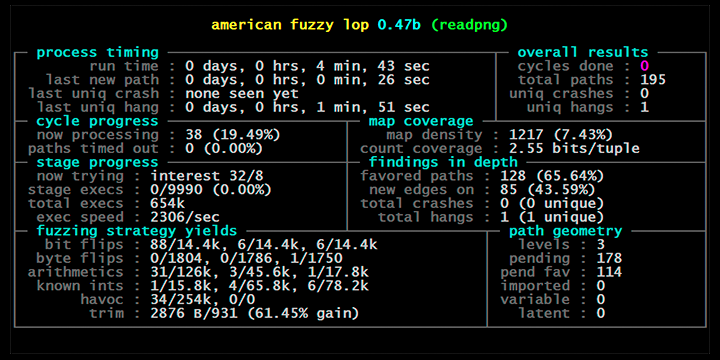
\includegraphics[width=\textwidth]{Chapter2/afl_screen.png}
    \centering
    \caption{AFL status screen}
    \label{fig:status_screen}
\end{figure} 

\begin{enumerate}
    \item \textbf{Process timing}: This section tells about how long the fuzzing process is running.
    \item \textbf{Overall results}: A simplified information about the progress of AFL in finding paths, hangs, and crashes. 
    \item \textbf{Cycle progress}: As mentioned before, AFL takes one input and repeats mutating it for a while. This section shows the information about the current cycle that the fuzzer is working on.
    \item \textbf{Map coverage}: \say{The section provides some trivia about the coverage observed by the instrumentation embedded in the target binary. The first line in the box tells you how many branches we have already hit, in proportion to how much the bitmap can hold. The number on the left describes the current input; the one on the right is the entire input corpus's value. The other line deals with the variability in tuple hit counts seen in the binary. In essence, if every taken branch is always taken a fixed number of times for all the inputs we have tried, this will read "1.00". As we manage to trigger other hit counts for every branch, the needle will start to move toward "8.00" (every bit in the 8-bit map hit) but will probably never reach that extreme. 
    
    Together, the values can help compare the coverage of several different fuzzing jobs that rely on the same instrumented binary.
    }
    \item \textbf{Stage progress}: The information about the current mutation stage is briefly provided here.
    \item \textbf{Findings in depth}: The crashes and hangs and any other findings (here we have the other information about the coverage) are presented in this section.
    \item \textbf{Fuzzing strategy yields}: To illustrate more stats about the strategies used since the beginning of fuzzing, and for comparison of those strategies, AFL keeps track of how many paths were explored, in proportion to the number of executions attempted, for each of the fuzzing strategies.
    \item \textbf{Path geometry}: The information about the inputs and their depths, which says how many generations of different paths were produced in the process. For instance, we call the seeds we provided for fuzzing the "level 1" inputs. Next, a new set of inputs is generated as "level 2", the inputs derived from "level 2" are "level 3," and so on.
\end{enumerate}

\subsubsection*{Command}

AFL requires the instrumented binary for execution. To start the instrumentation, AFL uses \textit{afl-clang}, which is built with the coverage recipe included. The following command instruments the sample program \ref{lst:sample_vul}:

\begin{lstlisting}[language=bash,style=CommandStyle,caption=Instrument $sample\_vul$.c]
    afl-clang sample_vul.c -o sample_vul_i
\end{lstlisting}

Now AFL can run this program in \textit{afl-fuzz} with the coverage instrumentations.

\begin{lstlisting}[language=bash,style=CommandStyle,caption=Execute AFL]
  # afl-fuzz -i <in_dir> -o <out_dir> [options] -- /path/to/fuzzed/app [params]
  afl-fuzz -i in_dir -o out_dir -- ./sample_vul_i
\end{lstlisting}

The fuzzing continues until the fuzz testing is stopped using a termination signal. Pressing \textit{Ctrl+C} is a common command for this purpose. All of the recorded information are accessed through the output directory \textit{out\_dir}.